% ##################################################################################################################
\chapter{Zürich}
\label{ch:zhscenario}
\hfill \textbf{Authors:} Nadine Rieser-Schüssler, Patrick M. Bösch, Andreas Horni, Michael Balmer

\editdone{This text has undergone the professional edit. Please no grammatical changes anymore! They are most-probably wrong.}

% ##################################################################################################################
The \gls{matsim} team frequently uses the Zürich scenario, based on the Switzerland scenario described above. The Zürich scenario, however, is more detailed; it was enhanced by data available only for the smaller region; \eg traffic light data or freight demand data was only included for Zürich city and the canton. It is under continuous development, calibration and validation and has been applied in numerous projects, serving as a real-world research example.   

\citet{HorniEtAl_TechRep_IVT_2011_a} provided a technical overview of the first scenario branch; \citet[][]{BalmerEtAl_ResRep_bdktzrh_2009} described its generation for the ``Westumfahrung'' project . 

The study area was delineated by a circle, with a 30\,kilometer radius around Bellevue, a central and prominent Zürich location. This delineation led to two versions,  the \emph{Zürich diluted scenario} and the \emph{Zürich cut scenario}. For the first, all agents crossing the study area during the simulated day were considered (Figure~\ref{fig:zurichScenario}), resulting in almost two million agents. For the second, only agents remaining in this area the whole day were modeled. The \emph{Zürich cut scenario} was employed as an experiment in \citet[][]{Hackney_PhDThesis_2009}, but using the \emph{Zürich diluted scenario} for production runs is preferable.

Demand was taken directly from the Swiss model; freight traffic was also added to the Zürich scenario, as follows. Canton Zürich raw freight traffic data was taken from the \gls{kvmzh}, provided by \citet{AMV_Webpage_2011} and documented in \citet[][]{GottardiBuergler_SV_1999}. Zonal level matrices were disaggregated to single \gls{matsim} plans \citep[][]{ShahM_TechRep_IVT_2010}. Matrices for small delivery and heavy trucks were combined into one activity called \emph{freight}. An additional 180\,000 agents were generated for the Zürich region.

For the diluted Zürich scenario, all Swiss facilities, as described above, were used as activity locations and the networks were not thinned out. For public transport simulation, network and transport schedules were derived from the \gls{kvmzh}. Walk and bike modes were ``\gls{teleported}''. 

Calibration was mainly done for modal split and distance distributions and utility function values set accordingly.

For validation, count data on city level, cantonal level and national level \citep[][]{ASTRA_Webpage_2006} were available from various sources, resulting in 123\,links measured for the Zürich inner city, delineated by a 12\,kilometer radius around Bellevue. The reduced count analysis radius was applied to reduce boundary effects resulting from demand reduction outside the 30\,kilometer radius study area. An average working day (Monday to Thursday, excluding public holidays) was used for comparison in current scenarios.

Some traffic signal data was available for Zürich city \citep[][]{STAPOZH-DAV_unpub_gtZH_2008}; this was integrated for the Westumfahrung project.
%
\createfigure%
{The diluted Zürich scenario}%
{The diluted Zürich scenario}%
{\label{fig:zurichScenario}}%
{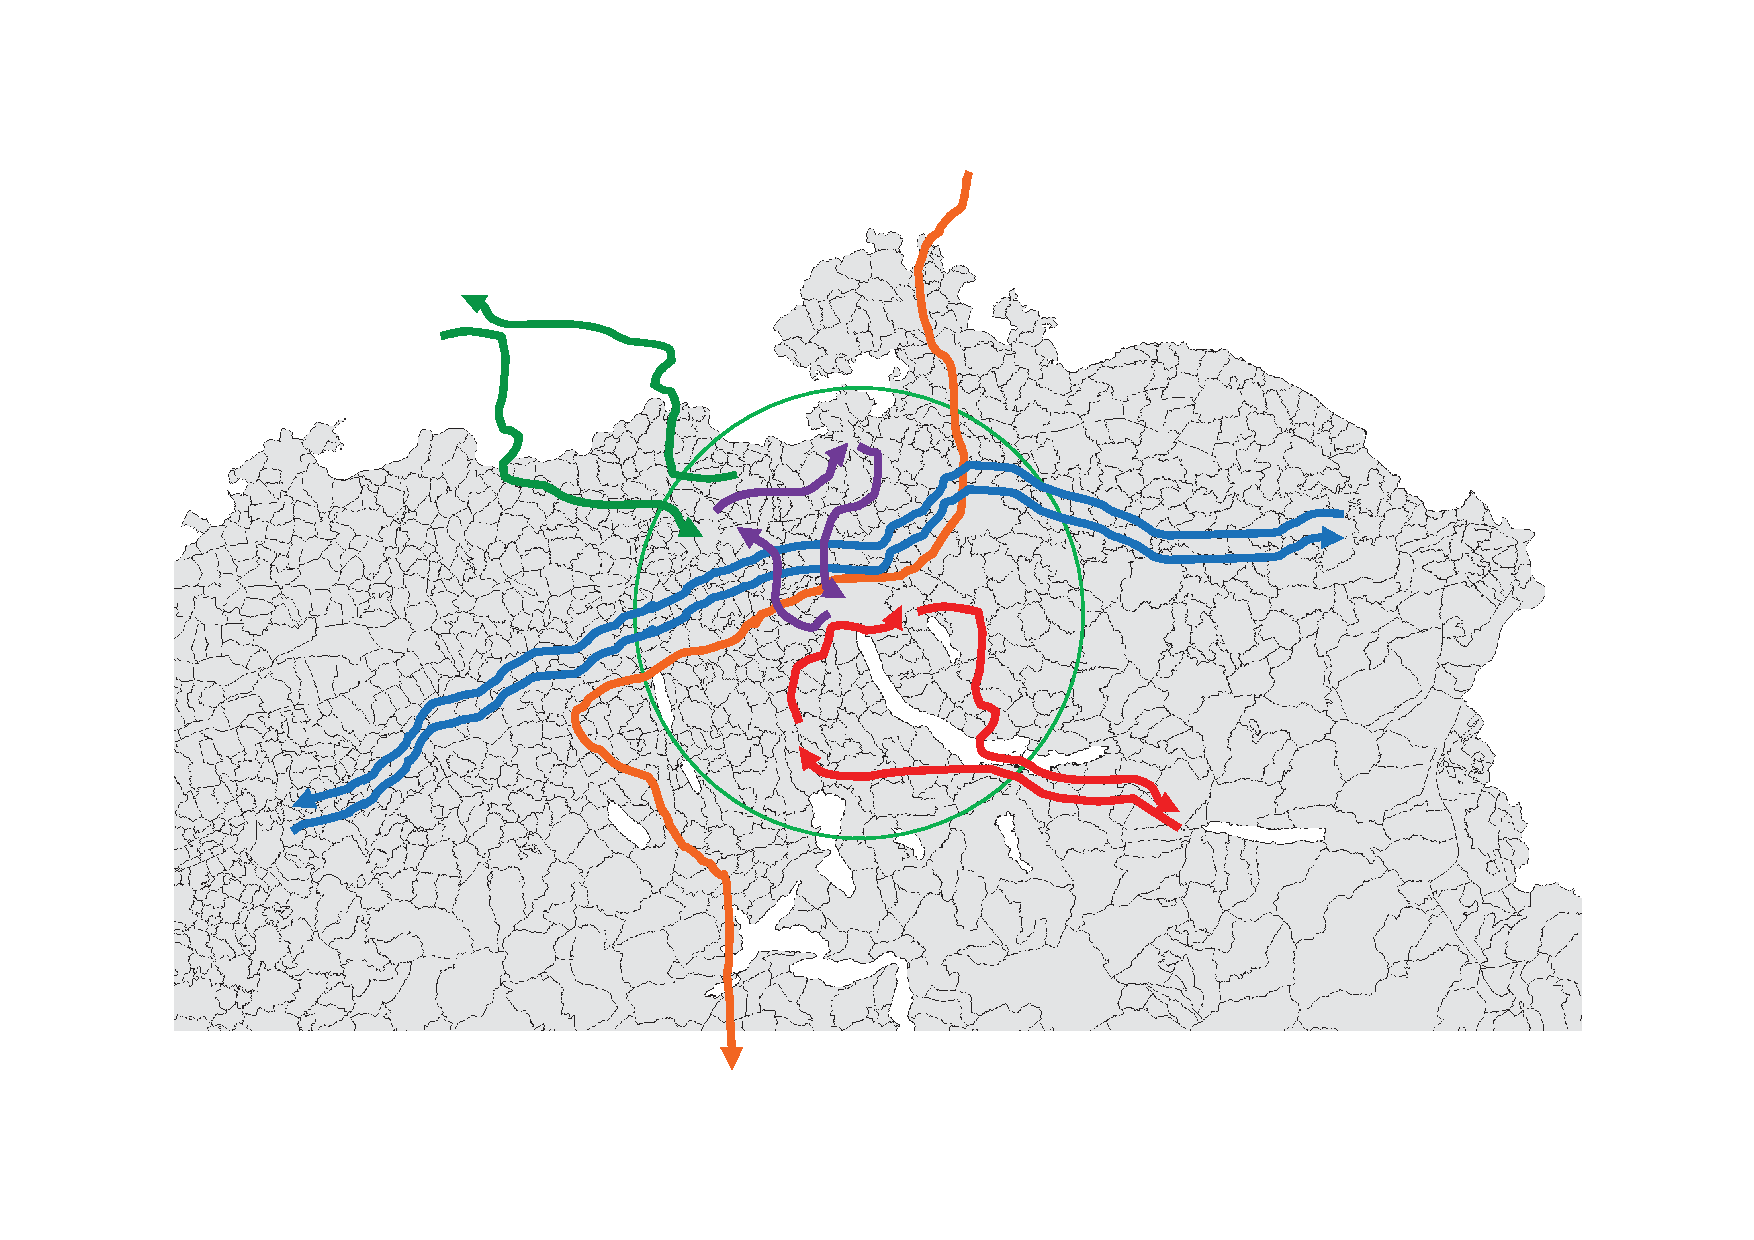
\includegraphics[width=0.99\textwidth, angle=0]{scenarios/figures/zh.pdf}}%
{}

% ##################################################################################################################
\section{Studies Based on the Zürich Scenario}
Besides its widespread use for the development of new \gls{matsim} functionality (\eg the contributions for destination innovation, joint decisions, parking or electric vehicles) the Zurich scenario has also been used in policy studies. 
The most prominent one was the study Westumfahrung \citep{BalmerEtAl_ResRep_bdktzrh_2009}, where \gls{matsim} was used to estimate the effects of opening a new motorway section and different accompanying measures. 
In addition to classic evaluations such as link volumes and spider analyses, the project focused on estimating who the winner and loser of the Westumfahrung were and where they lived. 
Other policy studies looked at the potential for Park \& Ride and organized as well as informal ride sharing, the effects of a substantially improved public transport offer and the influence of road capacity changes on transport behavior. 

%ToPDAd:
A more recent example for a study based on the Zürich scenario is described in \citet[][]{HeyndrickxEtAl_unpub_TRB_2016, BoeschEtAl_TechRep_ToPDAd_2014,HeyndrickxEtAl_TechRep_IVT_2014,PilliSihvolaEtAl_EJTIR_2014,BoeschCiari_STRC_2014,Boesch_unpub_MATSim_2014}. It was conducted as a part of the EU project \gls{topdad}. \gls{topdad} tried to find the best strategies for decision makers to adapt to the expected short and long term effects of climate change. The international project focused on the three potentially climate sensitive and important economic sectors Energy, Transport and Tourism.

For each sector different case studies were investigated to develop the tools required to find suitable adaptation strategies. In the transport sector the \gls{ivt} together with the \gls{tml}, Belgium, conducted a study on the potential influence of extreme weather events, which are predicted to increase in frequency and intensity for Western Europe due to climate change, on the transport system.

The Zürich scenario was used to identify the transport system reactions on different, weather-induced disturbances. The number of trips, activities, and their durations were compared for different scenarios. The applied scenarios represented variations both on a supply side and on the demand side. On the supply side, next to the baseline scenario eight different scenarios were simulated. A medium and a high disturbance scenario, where the capacity and the free-flow speed on the entire network were reduced due to unfavorable weather conditions and a medium and high disruption scenario where certain, exposed street and public transport links were (temporary) blocked. These disturbances and disruptions occurred only in the peak hour or for the full day, resulting in the eight scenarios on the supply side. On the demand side the agents were allowed five different degrees of flexibility to react to this situation: 1.~Worst case (no reaction allowed); 2.~Rerouting; 3.~Rerouting and modal change; 4.~Rerouting, modal change and rescheduling; and finally 5.~Rerouting, modal change, rescheduling and relocation.

It was found that rerouting and mode choice together have the highest impact in terms of reaction to the disturbances. If the public transport system is disrupted, the expected shift to car and slow modes is observed. The opposite, expected shift to increased pt-usage is also correctly observed if the transport system is disturbed by unfavorable weather conditions (\eg rain or snow).

The results of these scenarios were used by TML to calculate the direct and indirect economic costs of extreme weather events through an impaired transport system. Extreme events with a return value of five to ten years are estimated to cause costs of 0.2\,EUR to 19\,million\,EUR per event for the region of Zürich, while the more extreme events with a return value of only 50 to 100\,years would cause costs of 10\,EUR to 100\,million\,EUR per event. Compared to estimations for historic events these are relatively low values (costs of billions per event). One of the reasons for this difference is assumed to be in the inability of \gls{matsim} agents to drop activities. So, while in reality people would for example likely drop work activities in the case of severe floods and thus cause additional economic costs, \gls{matsim} agents will always try to find a way to get to their work location and to work – no matter how bad the circumstances. Current efforts at IVT try to overcome this limitation while still producing realistic simulation outcomes.

% ##################################################################################################################






